\documentclass{nime-alternate}
\usepackage{url}
\usepackage{graphicx, color}
\begin{document}

\numberofauthors{1}
\title{Peacock III: The development of an autonomous non-haptic performance instrument}
\author{
\alignauthor
Chikashi Miyama\\
       \affaddr{College of Music and Dance Cologne}\\
       \email{me@chikashi.net}
}

\maketitle
\begin{abstract}
Peacock is a box-shaped instrument for musical performances. The instrumemnt is equipped with thirty-five proximity sensors arranged in five rows and seven columns. The sensors detect the movements of a performer's hands and arms in a three-dimensional space above them. Peacock III, the newest version of Peacock features a small embeded digital synthesizer, a multi-thread dedicated application, and gesture recognition system that provide compoers and improvisers with more intimate interactions between human body and electronic sound. 
\end{abstract}

\section{Background and the issues of previous version of Peacock}

\begin{figure}[htbp]
       \begin{center}
              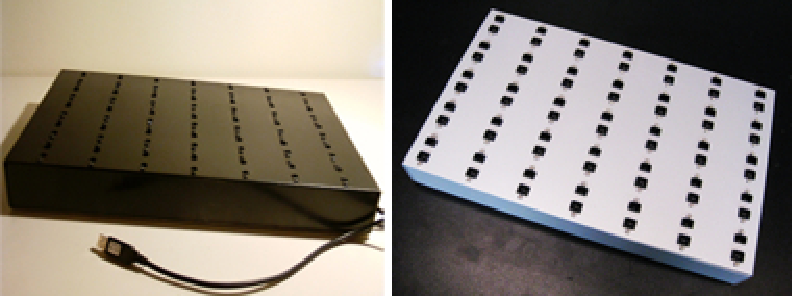
\includegraphics[scale = 0.55]{Peacocks.pdf}
       \end{center}
       \caption{Peacock I and II}
       \label{fig:old_peacock}
\end{figure}

Peacock I, the first model of Peacock series, was developed by the author in 2009\cite{miyama:peacock}. It is a musical interface, equipped with 35 infrared proximity sensors that detect the movement of performer's hand and send them to a host computer, running a Pure Data\cite{Pd} patch for sound synthesis. This interface enables a performer to control 35 musical parameters, such as pitch, loudness, and timbre, in realtime without touching or wearing physical devices. Through three years of musical practice with Peacock I, several points for improvements were found:

\begin{enumerate}
\item The bandwidth of the data transfer from the microcontroller to the host computer (ca' 60 Hz.) is not sufficiently high and it causes recognizable latency.

\item The infrared proximity sensors, employed for Peacock I (Sharp GP2D12), detect obstacles in the range only from 10 to 80 cm. This restrict performers from using entire available vertical space with his/her hands above the instrument. 

\item Since the interface should be connected to a host computer by a USB cable for sound synthesis, a laptop computer must be placed next to the interface. This restricts the autonomy and the mobility of the device, as a musical instrument.

\item The S/N ratio of the analog data from the infrared sensors is not sufficiently high. The data contain significant amount of analog noise and it interferes with the precise paramter control by hands.

\item The main circuit board of Peacock I is soldered on a single universal board; the cost and labor for the reproduction poses a difficulty in the realization of duo, trio, or ensemble performances with multiple Peacocks.

\item Peacock I simply detects the distance between 35 infrared sensors and hands and allows us to map these data to musical paramters; By analyzing incoming data, it would be possible to obtain more abstract data, such as the  positions of the hands, the centroids, the speed of movements, and the trajectories of the hands (i.e. gestures). These data can be also utilized as sources of parameter control or as musical commands.

\end{enumerate}

In 2011, this project received a DAAD research scholarship and Peacock II, a new version of Peacock, was realized at ZKM, Karlsruhe, Germany. The new version solves the first two issues mentioned above by using , faster microcontroller\cite{parallax:propeller} and alternative infrared sensors.


\section{Peacock III}

Though Peacock II is a significant improvement, there are still four issues. This paper introduces the features of the newest version of the seires, {\bf Peacock III}, that overcomes these four issues. 


In order to improve the autonomy and mobility of the device, a small computer for the audio synthesis is embedded in the enclosure of Peacock III. It enables users to use Peacock without connecting it to an external laptop for audio synthesis; Peacock III can be employed as an autonomous electronic instrument, such as an electric guitar or a keyboard synthesizer. 

Furthermore, a PCB (Printed Circuit Board) is designed as a solution to the fourth and fifth issues. The PCB  denoises the signal from the sensors with hardware lowpass filters, and reduces the cost and the labor for the reproduction significantly. 

As a solution for the last issue, a C++ program was developed for gesture recognition; it analyzes the incoming data, detects the hand gestures, and allows us to map the results of the analysis onto musical parameters and commands.

\section{System overview}
\begin{figure}[htbp]
       \begin{center}
              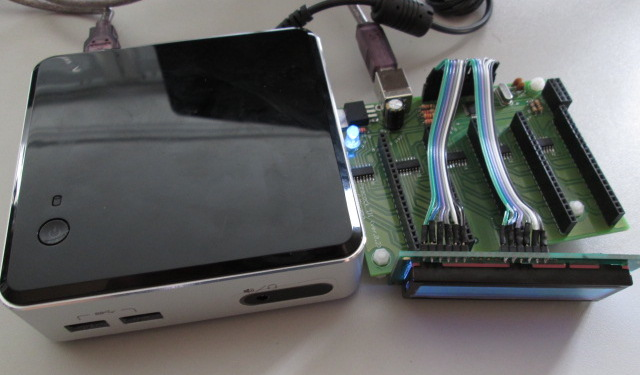
\includegraphics[scale=0.9]{interface_main.jpg}
       \end{center}
       \caption{main unit and interface board}
       \label{fig:interface_main}
\end{figure}

The Peacock hardware mainly consists of two components;\\
\textbf{main unit} and \textbf{interface board}. The interface board is a 100mm x 60 mm-sized PCB(printed circuit board), that collects the data from all 35 sensors, digitize them, and forward them to the main unit. It is also equipped with four buttons and a text LCD that enables users to operate Peacock system and indicates the current status of the system.

The main unit, an embeded small computer (102 mm x 102 mm) in the enclosure, analyzes the incoming data from the interface board, maps them onto the parameters of software synthesizers, and generates sound. Optionally, the main unit visualizes the incoming data.


\section{Interface Board} % (fold)

\begin{figure}[htbp]
       \begin{center}
              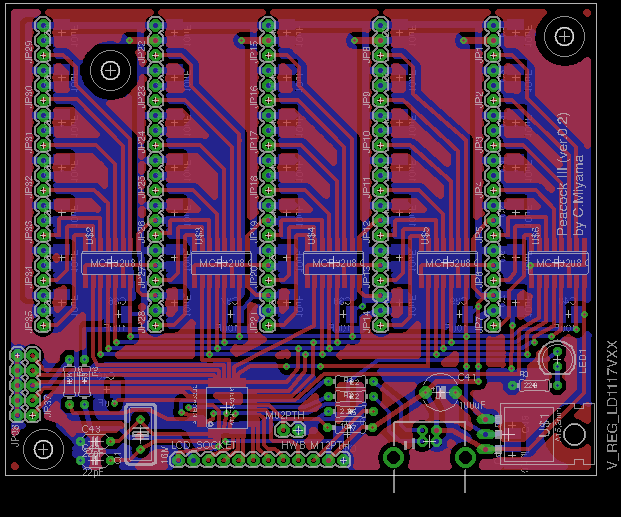
\includegraphics[width=1\columnwidth]{board}
       \end{center}
       \caption{The PCB of Peacock III}
       \label{fig:board}
\end{figure}

The interface board comprises an ATMega 32U2 microcontroller\cite{atmel:avr}, five external 12 bit ADCs, a text LCD, 4 buttons and a LED. The main functionalities of the interface board are as follows:

\begin{enumerate}
       \item stabilization of the sensor power supply, employing onboard capacitors
       \item digitization of the signal from sensors with 5 external ADCs
       \item to provide interfaces for basic operation of the system with the buttons
       \item status indication of the system, using the connected LCD
       \item data transfer to the main unit via a USB cable, employing LUFA framework
\end{enumerate}

\begin{figure}[htbp]
       \begin{center}
              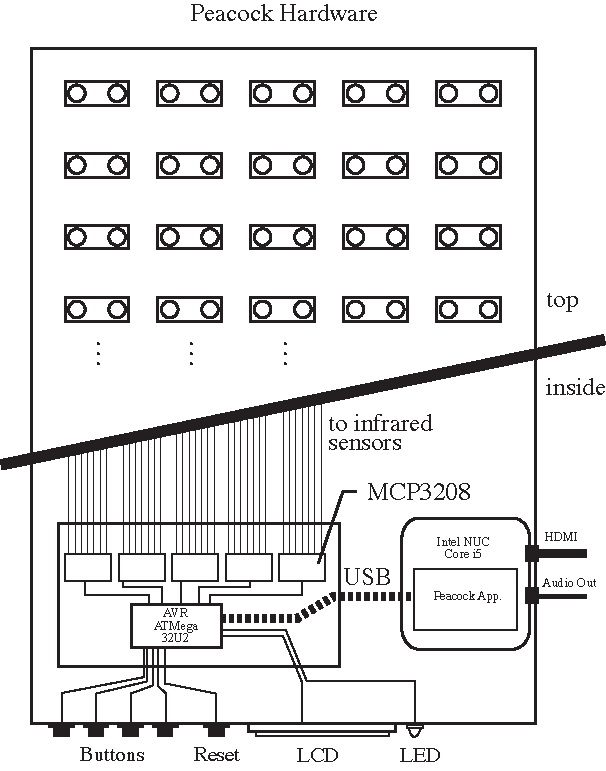
\includegraphics[width=1\columnwidth]{Peacock_hardware.pdf}
       \end{center}
       \caption{The Peacock III Hardware}
       \label{fig:peacock}
\end{figure}

\subsubsection{Hardware signal stabilization} % (fold)
The signal from infrared proximity sensors employed by Peacock include significant amount of noise. In the previous version of Peacock, the signal was denoised in the software by applying digital low pass filters to all incoming digital data. However, The PCB of Peacock III is equipped with capcitors for each infrared sensor for stabilizaing its power supply. Since the noise is caused by the rapid current draw that result from pulsations generated by the emitter of the infrared sensors, The stabilization of the power supply removes a significant amount of noise from the analog signal.

\subsubsection{data collection} % (fold)
In order to collect data from all 35 infrared sensors, five 8 channel 12 bit A/D converters(MCP3208) are installed on the board and they communicates with AVR ATMega 32U2, the main microcontroller on the interface board, using SPI(Serial Periferal Interface) protocol. In the microcontroller, the collected data are packed in 39 bytes long serial packets, consisting of one byte of start delimeter, end delimeter, message ID, check sum and 35 bytes of actual data from the sensors.

\subsubsection{Status indication/manipulation} % (fold)

A 2x16 text LCD is attached on the side panel of the enclosure and it displays current status of the system. Users are capable of changing the setting of the system, and control the program for the sound synthesis, using buttons, attached next to the buttons.

\subsection{transfer of the data packets} % (fold)

In Peacock I, a FTDI chip bridges the UART messages from the AVR microcontroller to the host computer.
However, by employing AVR ATMega 32U2, a microcontroller with a hardware USB controller, Peacock III is capable of sending data directly from the microcontroller to the host computer. For the development of the USB-compatible firmware, LUFA (Lightweight USB Framework for AVRs)\cite{camera:lufa} was employed. The host computer recognize the Peacock PCB as a virtual serial device and receives data packet more than 1000 time per seconds. The speed of data transfer is also configurable by the buttons.

\section{Main Unit} % (fold)
The Main Unit, a dedicated embedded Intel NUC computer\cite{intel:nuc} is placed next to the PCB board in the enclosure.

\subsection{Peacock App}

This computer runs Arch linux and {\bf PeacockApp} on it. \\
PeacockApp is an openFrameworks\cite{openframeworks}-based program written in C++. This application receives the data from the microcontroller and forwards it to the three sub-modules listed below. 

\begin{enumerate}
       \item Gesture Recognizer(PckRecognizer)
       \item Synthesizer(PckSynthesizer)
       \item Visualizer(PckVisualizer)
\end{enumerate}

In order to minimize the latency and maximize the efficiency of the data processing, These three modules runs on three separate threads in PeacockApp. If the {\it Gesture Recognizer} module detects a certain hand gesture, a notification will be sent immediately to the other two modules.

\begin{figure}[htbp]
       \begin{center}
              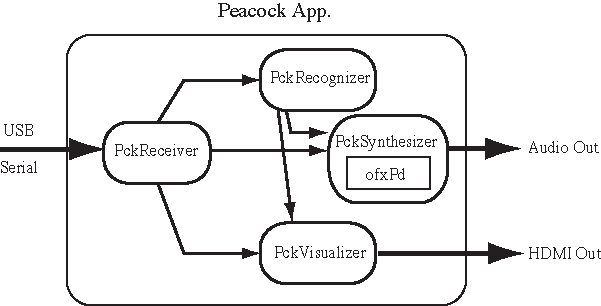
\includegraphics[width=1\columnwidth]{Peacock_app.pdf}
       \end{center}
       \caption{The Peacock III App}
       \label{fig:modules}
\end{figure}

\subsubsection{Gesture Recognizer: PckRecognizer}

The {\it Gesture Recognizer} modules currently detects, the presence and number of hands above the hardware, the estimated position of two hands, and the centroid of each row and column. 
If this module find some new infomation, notifications to other two modules will be immediately sent\ref{fig:modules}.

\subsubsection{Sound Generator: PckSynthesizer}

The sound generator module is programmed with Pd\cite{Pd}. ofxPd\cite{ofxPd}, an Pd addon for oF\\(OpenFrameworks), enables the PeacockApp to run Pd patches within it. The Pd patches receives all data from the sensors, the result of analysis by the Gesture Recognizer, and the commands from buttons on the side panel. All these data can be mapped to any musical parameters.
 
\subsubsection{Visualizer: PckVisualizer}

Unlike piano, cello, or other acoustic instruments, the player of Peacock controls musical parameters by simply moving hand above the device; There is no physical feedback from the instrument. In order to improve accurate parameter control by the performer, a visualizer is developed.  The visualizer indicates the values of from 35 infrared sensors  the assumed position of hands, chronological trail of hand movement, and recognized gestures, in  3D model programmed with OpenGL\cite{OpenGL}. The renderered 3D images can be displayed by attaching an optional HDMI-compatible monitor to the device.
The visualizer can be deactivated by the user by the attached buttons.

\begin{figure}[htbp]
       \begin{center}
              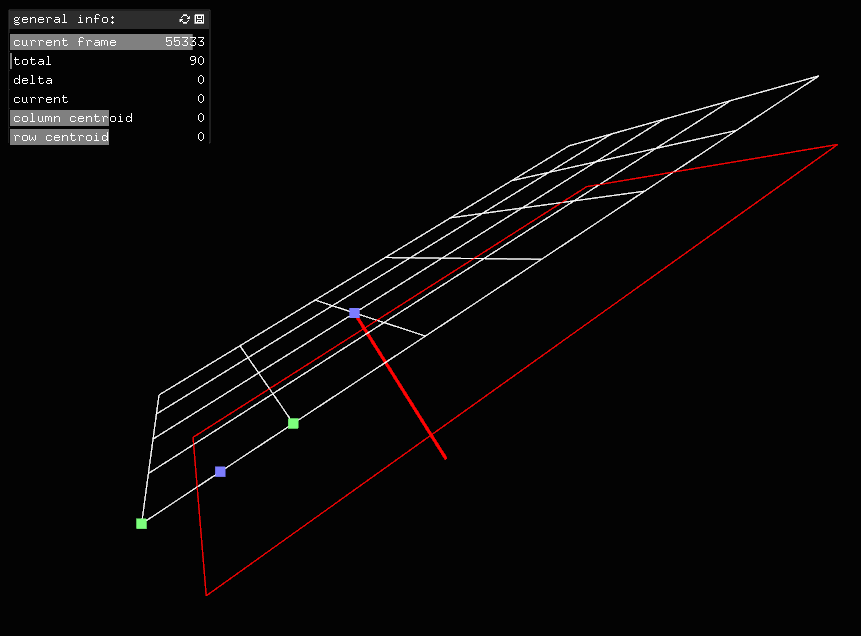
\includegraphics[scale=0.3]{visualizer.png}
       \end{center}
       \caption{Visualizer}
       \label{fig:visualizer}
\end{figure}


\section{future works}

Further improvement of firmware and in the PeacockApp module is scheduled.
The source code of the PeacockApp and Peacock Firmware is hosted on github.com under GPL v3 lincense.


\section{acknowledgement}
This project is funded by fellowship program of the Academy of Media Arts Cologne. The author would like to express a sincere appreciation to Prof. Anthony Moore and Mr. Dirk Specht for their valuable support.

\bibliographystyle{abbrv}
\bibliography{KHM-references.bib}

\end{document}
